\subsection{A4 Staff Criterion}

The school leadership and staff are qualified for their assigned responsibilities, are committed to the school’s purpose and engage in ongoing professional development that promotes student learning in a global society.

\subsubsection{Employment Policies/Practices and Qualifications of Staff}

\indicator{The school has clear employment policies/practices related to qualification requirements of staff.The school reviews all information regarding staff background, training, and preparation, including international expertise.}

\prompt{Evaluate the clarity of the employment policies and practices related to qualification/statutory requirements of current and potential staff for all programs, including all types of online instruction and specialized programs such as college/career preparation.}

\begin{findings}
CMIS has always recognizes the need to hire suitably qualified people to fill its administrative, teaching, and non-teaching positions. After extensive research from the educational organizations CMIS has membership to:

\begin{itemize}
\item The International School Association of Thailand (\href{http://gallery.cmis.ac.th/2016-2017/ISAT-Regional-Meeting/}{ISAT})
\item The East Asia Regional Council of Schools (\href{https://www.earcos.org/}{EARCOS})
\item Association of Christian Schools International (\href{https://www.acsi.org/}{ACSI})
\item The Association for Supervision and Curriculum Development (\href{http://www.ascd.org/about-ascd.aspx}{ASCD})
\item Academy for International School Heads (\href{http://aishbank.squarespace.com/}{AISH})
\item National Association of Independent School (\href{http://www.nais.org/Pages/default.aspx}{NAIS}) 
\end{itemize}

The School management team realized that some of their policies were outdated and did not reflect current research, especially in terms of global competency. Beginning 2016-17 school year they developed more defined employment policies and practices of potential staff:

Current Requirements:
\begin{itemize}
\item Current certification in home country
\item Original documentation verifying credentials
\item 3 confidential reference checks
\item First interview with immediate supervisor/team
\item Second interview with Superintendent and Principal
\item Third interview with SET
\item Clearance of criminal background check
\item Signed agreement to child abuse policy
\item Signed agreement to contractual obligations
\item Completion of new staff orientation
\item Completion of probationary period
\end{itemize}

These requirements are outlined in the \href{http://cmis.ac.th/about/employment}{employment section} of the CMIS website and on the our recruitment sites (e.g., The International Educator). CMIS believes that student learning benefits greatly from a highly qualified and trained team, and school leadership is committed to continuing to recruit highly qualified and effective staff to advance the school’s purpose and core values.

The updated expectations have required some of our existing staff to renew their certification and clearance documentation. ALL staff are currently in the process of doing so with the support and guidance of the Human Resources department.

\minor{So what...}

CMIS has worked hard to improve and strengthen their employment strategies. Their efforts have solidified the need to remain up to date with global employment practices that focus on recruiting practices that obtain and retain the most capable staff.
\end{findings}

{\centering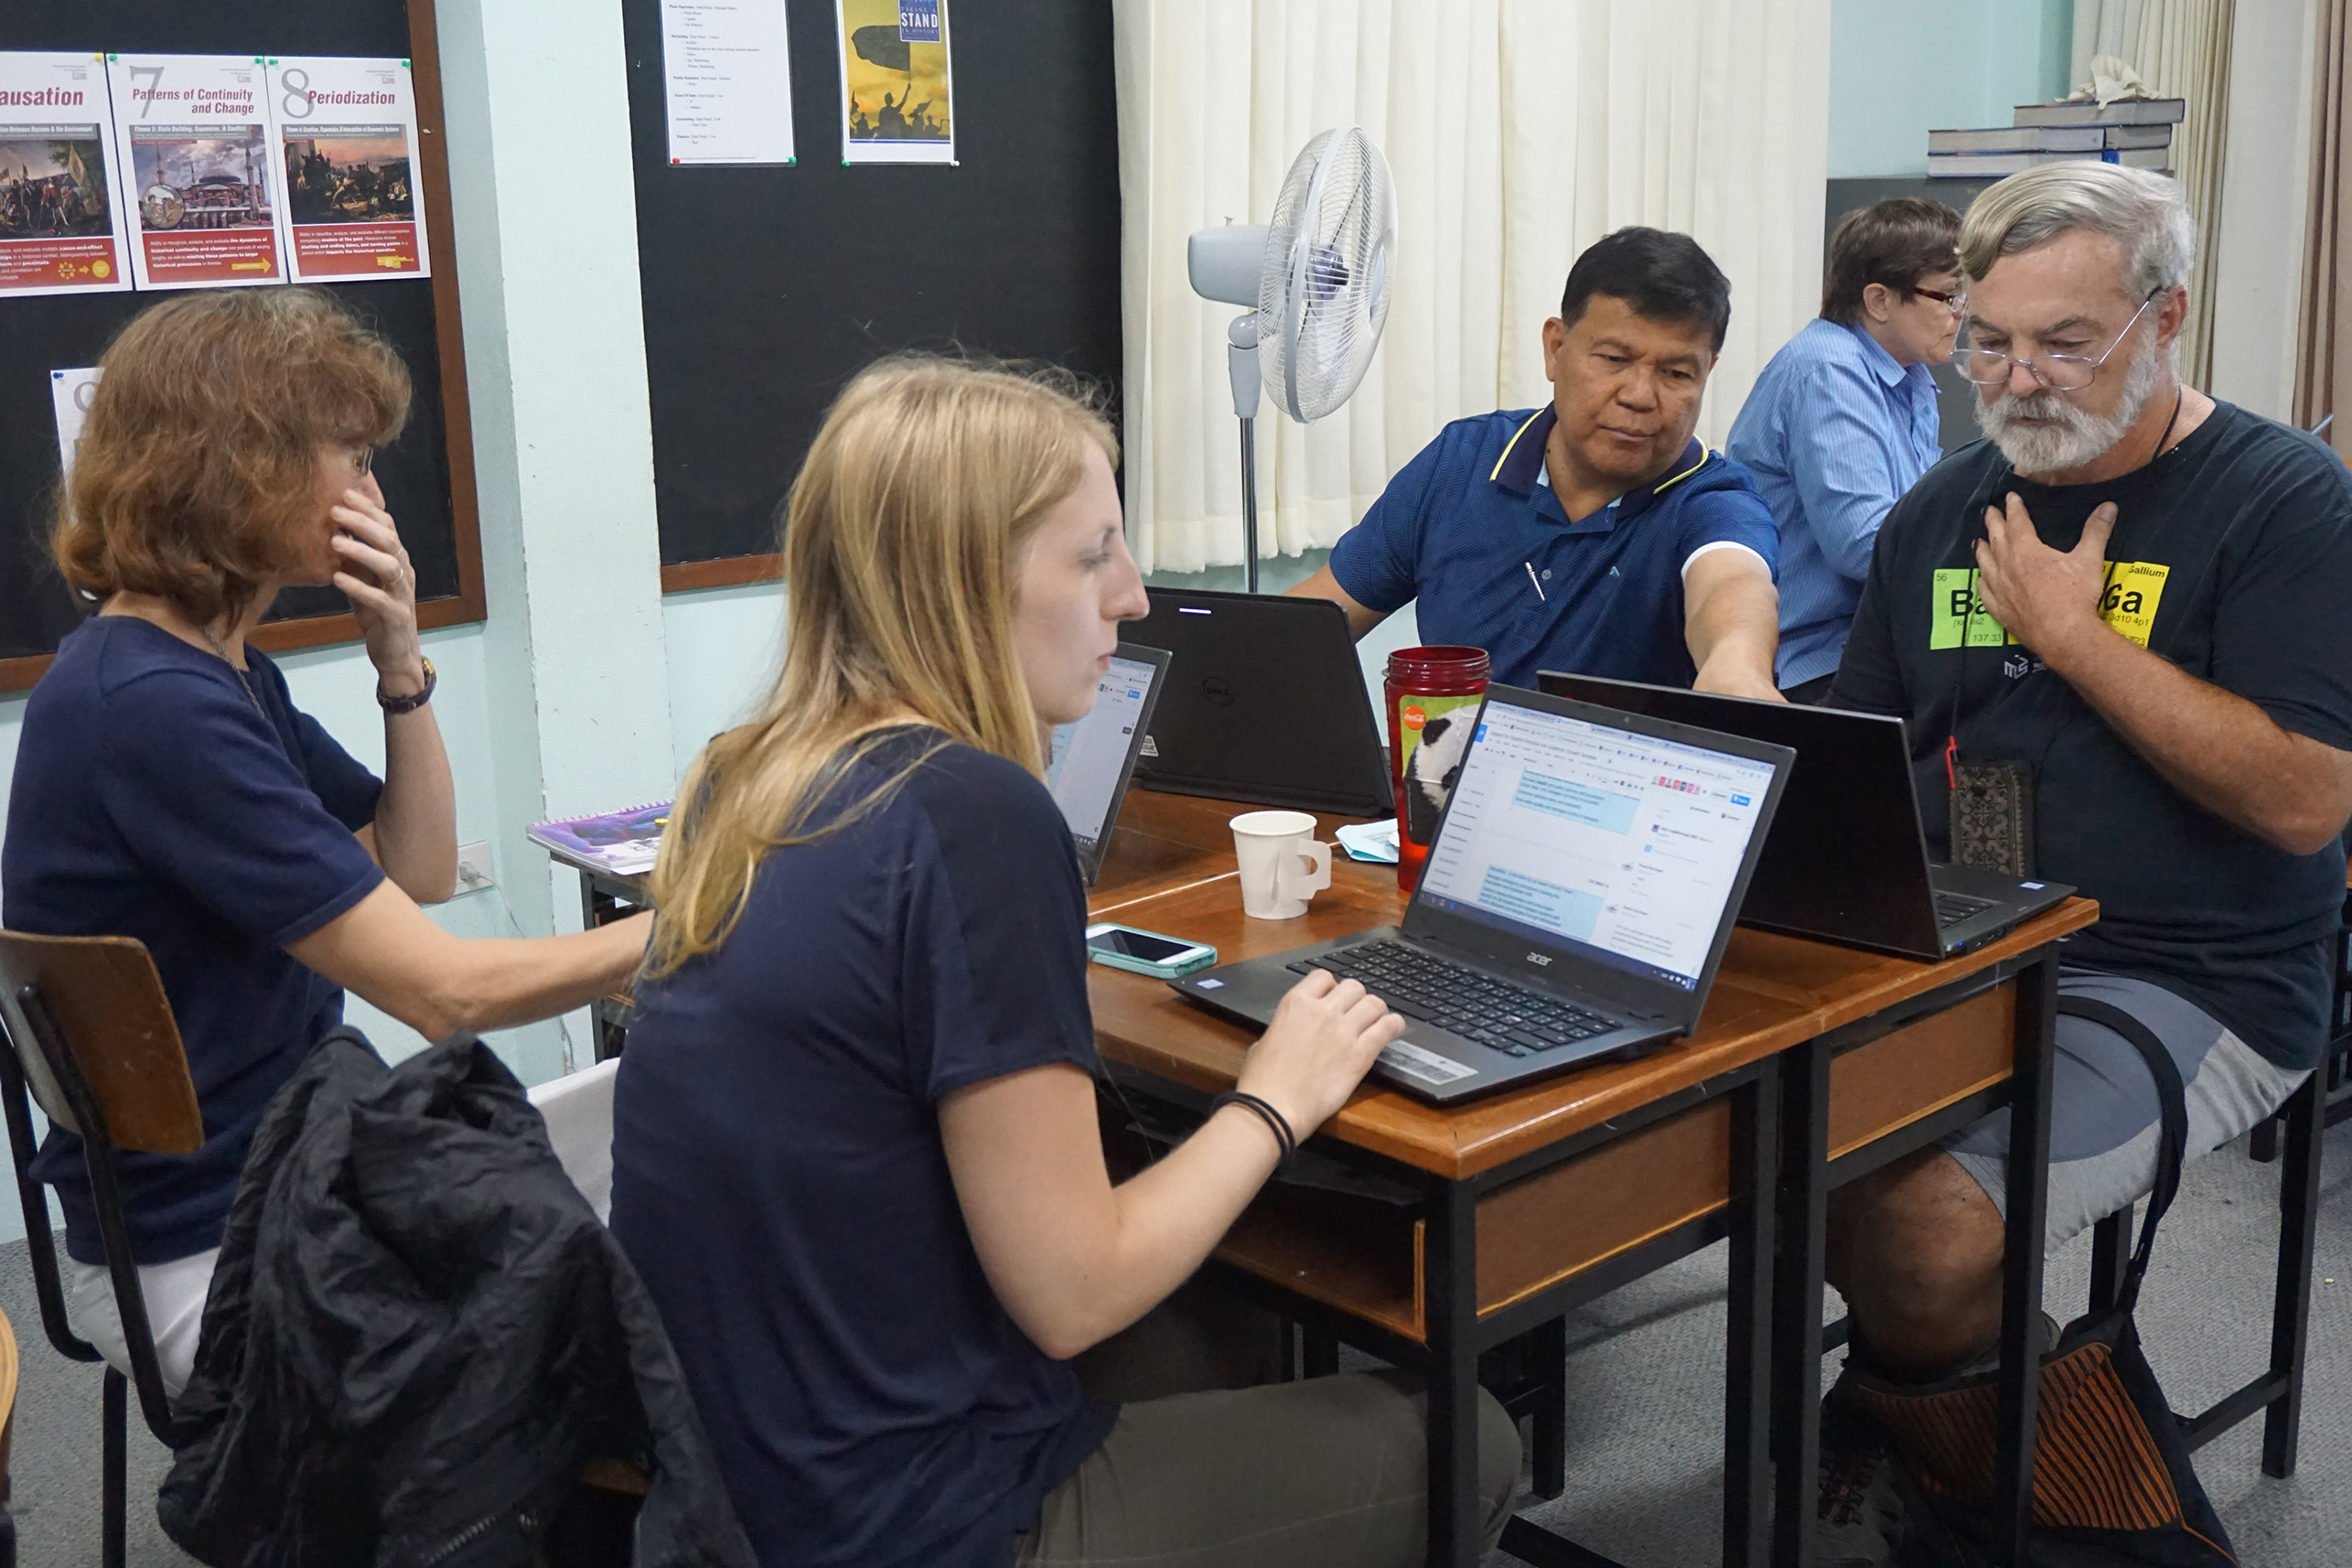
\includegraphics[width=\textwidth]{chapter4_a4.JPG}}
 
\subsubsection{Maximum Use of Staff Expertise}

\indicator{The school has a process to assign staff members and provide appropriate orientation for all assignments, including online instruction and specialized programs so that the expertise of the staff members is maximized in relation to impact on quality student learning.}

\prompt{Evaluate the process to assign staff members and provide an appropriate orientation process to ensure all staff are qualified and prepared or their responsibilities including any type of online instruction}

\begin{findings}
In 2015-2016 school year an Human Resources and Registrar position was created to assist staff with additional support  and guidance.During the 2016-17 school year an additional Human Resources assistant position was enlisted to create an Human Resources department. As well as help with salaries and benefits, this department also assists staff and parents with visa, permit, and governmental requirements.

Last year, CMIS established a New Staff Welcoming Committee. The main objective of this committee  was to create a smooth transition for all new staff and help them prepare all necessary paperwork and documentation. In addition, new staff members were provided with 5 days accommodation at on-site housing in an effort to improve the transitional period especially as the majority of our new hires are travelling from different countries.

This year, CMIS created a New Hire Buddy Program where current staff volunteer to “adopt” a new hire in an effort to make the personal transition to Chiang Mai as seamless as possible. New staff  are also assigned a Team Leader to assist them with curriculum and instructional support. Starting last year, new hires begin the school year a week earlier than returning staff to participate in New Staff Orientation programs and a Thai Culture training curriculum.

Based on feedback from new staff, the 2016-17 New Teacher Orientation was extended to include more time to work in classrooms, plan with colleagues, and manage personal needs (e.g. accommodation and travel)

Based on feedback from new staff, the Returning Staff Orientation has been modified to include  more opportunities for returning staff to collaborate with new faculty, receive training updates (e.g. Data wise, Ubd, Powerschool etc.) and work within their departments.

\minor{So what...}

CMIS worked hard to increase the opportunities for appropriate orientation to all staff. We understand that this additional support increases the expertise of the staff members is maximized in relation to impact on quality student learning. CMIS leadership believes that they can increase these opportunities further and are currently working with staff to explore additional ways.
\end{findings}Findings

\subsubsection{Defining and Understanding Practices/Relationships}

\indicator{The school has clear administrator and faculty written policies, charts, and handbooks that define responsibilities, operational practices, decision-making processes, and relationships of leadership and staff.}

\prompt{Evaluate the administrator and faculty written policies, charts, pacing guides and handbooks that define responsibilities, operational practices, decision-making processes, and relationships of leadership and staff. Determine the degree of clarity and understanding of these by administration and faculty.}

\begin{findings}
CMIS has clear written policies and \href{https://drive.google.com/a/cmis.ac.th/file/d/0Bwny3HLdIIS7RF9veFk5UXB2Q2M/view?usp=sharing}{organizational charts} that define responsibilities, operational practices, decision-making processes, and relationships of leadership and staff. These policies and procedures are reviewed and updated at the beginning of the year with all staff during the staff orientation.

Additional procedures and expectations can be found in the \href{https://docs.google.com/a/cmis.ac.th/document/d/1DrXVXsgw4U62HCGOceOKsgC8V1LDQFhHKgDB35oq4wY/edit?usp=sharing}{Faculty Handbook} which is updated and made available to staff as a Google document on a yearly basis. Policy and procedural updates are communicated during staff orientations, department, team leader and divisional meetings.

\minor{So what...}

CMIS understands the importance of having clearly written policies, and handbooks that define responsibilities, operational practices, decision-making processes, and relationships of leadership and staff. 

The CMIS faculty handbook has grown considerably in volume over the last few years and recent staff feedback has indicated that it can be difficult to navigate. In an attempt to address this concern the administration and team leaders have been working together to create a more streamlined and useful  2017-18 edition. 

Staff feedback (from TACT) this year indicated that the \href{https://docs.google.com/a/cmis.ac.th/presentation/d/18ekiAcUSiwa7oJM9tdwe2OSfnC_47RkbLz8ZjEt6O9I/edit?usp=sharing}{policies update presentation} this year was overwhelming for some staff and when presented as a whole group it was not conducive to open discussion. The leadership appreciated this feedback and apologized in person to the staff and resolved to present next year's presentation in small groups and in segments. 
\end{findings}

\subsubsection{Staff Actions/Accountability to Support Learning}

\indicator{The school evaluates the effectiveness of the processes and procedures for involving staff in shared responsibility, actions, and accountability to support student learning throughout all programs. This includes an evaluation of the collegial strategies used to implement innovations and encourage improvement, such as shadowing, coaching, observation, mentoring, and group presentations.}

\prompt{How effective are the processes and procedures for involving staff in shared responsibility, actions, and accountability to support student learning throughout all programs? Provide representative examples and data regarding impact on student learning.}

\begin{findings}
CMIS Leadership has provided processes and procedures to address shared responsibility and accountability. 

\minor{Collaborative Structures}

CMIS Leadership provides time for professional development and collegial discussions through the scheduling of meetings throughout the calendar year. Teachers meet as whole staff, department, divisional, and a Teacher Leadership Team to discuss different topics (e.g. integration, looking at student work, unit planning, cohesion, best practices etc). Whole staff meetings are normally reserved for specific professional development training. 49 out of 59 responses to the last professional development survey responded that the topics presented: 

\begin{itemize}
\item positively challenged the way [they] approach instruction, assessment, and planning; 
\item strengthened [their] understanding and application of instruction, assessment, and planning or; 
\item provided [them] with a solid foundation in which to grow my understanding of the topics.
\end{itemize}

See \href{https://docs.google.com/a/cmis.ac.th/forms/d/1-00JLey-jyLuizymm8z8JGJ6iLp4l-ccsTgHJ_Ckcj8/viewanalytics}{Professional Development Reflection} for more information. 

During the 2014-2015 school year, a great deal of professional development time was used to discuss and unpack the new literacy standards. One of the most critical design considerations of the standards is that they are a shared responsibility of all staff members. Each teachers, regardless of what they teach, have literacy standards. This discussion manifested into practice by adding key literary elements to the UbD unit template that all teachers must complete. See \href{http://www.corestandards.org/ELA-Literacy/introduction/key-design-consideration/}{Key Design Considerations} for more information. 
		
\href{https://docs.google.com/a/cmis.ac.th/presentation/d/1j9DjUPHbIprWWbftcBxiF35BKmzU5C_lW9Z78f8CAeE/edit?usp=sharing}{\minor{Instructional Rounds}}
The peer observation process provides another opportunity to involve staff in actions to address and support student learning. Instructional Rounds asks teachers to collect observational data on their colleagues, based upon a focus question that the teacher being observed chooses. By keeping the process free from evaluation and judgements, many teachers were able to view their practice objectively. The feedback was very positive. Some of the comments from participants include:

``It was a positive experience seeing my colleagues teach for the first time in five years”
``Having feedback from co-teachers is always helpful''
``Thanks for creating an environment/atmosphere that is non-threatening''
``Great to see other classes, get ideas from colleagues on student engagement''
``Inspired more and deeper conversations on what’s ‘measurable’''
``It genuinely answered a question that I could not effectively answer myself'' 

\minor{So what...}

Though CMIS uses processes and procedures to engage staff in shared responsibility, actions, and accountability, more time should be devoted to obtaining examples and data regarding impact on student learning.
\end{findings}

\subsubsection{Support of Professional Development}

\indicator{The school effectively supports professional development/learning with time, personnel, material, and fiscal resources to facilitate all students achieving the academic standards and the schoolwide learner outcomes. Teachers are involved in experiences such as visits, exchanges, and professional development to strengthen their understanding of global competencies.}

\prompt{How effective is the support of professional development/learning with time, personnel, material, and fiscal resources to facilitate all students achieving the academic standards and the schoolwide learner outcomes? Provide evidence and examples.}

\begin{findings}
The CMIS Leadership Team supports teacher professional development in a variety ways and is guided by current research. 

See the sections in the Curriculum, Instruction, and Assessment category entitled, Professional Collaboration and the Professional Development for details on how CMIS promotes and implements professional development opportunities. Subsections of the Professional Development indicator includes:

\begin{itemize}
\item Backed by Research
\item Early Release Wednesday
\item Consistency 
\item Outside Presenters
\item Chiang Mai Circle of International School (CMCIS) 
\item Other Professional Development Opportunities
\item Outside Professional Development 
\item CMIS Professional Development Fund 
\end{itemize}

\minor{So what...}

As noted in the Curriculum, Instruction, and Assessment category, professional development at CMIS is a priority. Though CMIS Leadership and Staff will continue to focus on reflective, genuine, deliberate teacher training, how the leadership and staff transition this information to the classroom and what accountability measures should be in place will continue to be a goal in the near future.
\end{findings}

\indicator{The school supports professional learning of the staff members that develops their use of important skills that are inherent in developing the global competencies of the students; these include collaboration, communication, creativity, and problem-solving.}

\prompt{Evaluate the effectiveness of the professional learning in relation to global competency skills being applied in individual classes and the learning results.}

\begin{findings}
CMIS Leadership supports professional development for staff that helps them support student collaboration, communication, creativity, and problem solving.

Teacher professional development at CMIS uses discussion protocol and structures to promote staff collaboration, communication, creativity, and problem solving. The facilitators review and encourage the teaching staff to use those protocols in their classrooms to promote the practice of these global competency skills. The following is just a sample of the different protocols that have been shared:

\begin{itemize}
\item save the last word,
\item appointment clock 
\item notices and wonderings
\item warm and cool feedback
\item passion profiles
\item hopes and fears
\item STR (Stop, Think, and React)
\item circle of voices
\item world cafe
\end{itemize}

The CMIS leadership have also provided professional development workshops to develop students problem solving skills. These workshops included What is Productive Failure? (2014), Language and Learning in Math (2015), and Focus, Coherence, and Rigor in Mathematics (2016)

\minor{So What...}

CMIS has been fortunate enough to have some teachers attend quality professional development.  CMIS will continue to monitor and maintain professional development requests to ensure that they are addressing not only the standards, but indicators of global learning.
\end{findings}

\subsubsection{Supervision and Evaluation}

\indicator{The school implements effective supervision and evaluation procedures in order to promote professional growth of staff in 21st century skills and thinking. Teachers regularly reflect on their approaches to develop global competencies in the students.}

\prompt{How effective are the school’s supervision and evaluation procedures?}

\begin{findings}
CMIS utilizes effective supervision and evaluation procedures in order to promote professional growth of staff in 21st century skills and thinking. Teachers regularly reflect on their approaches to develop global competencies in the students.

During the 2014-2015 school year the \href{https://docs.google.com/document/d/15_5X5QtixmWVheEUBVO9N1aislsLDm_ZW4-4g4YQ7F4/edit?usp=sharing}{CMIS Teacher Observation Tool} was modified and updated to include the findings of the research based report, \href{https://drive.google.com/a/cmis.ac.th/file/d/0Bwny3HLdIIS7bXJ0dEpCWG51MTQ/view?usp=sharing}{Essential Practices of High Quality Teaching and Learning}. The study analyzed recent educational literature an existing rubrics and frameworks that focus on the practice of effective teaching, and constructed a list of core, essential practices of high quality teaching and learning that cuts across all content areas and grade levels. 

The CMIS teacher evaluation process was also updated to include a more comprehensive self reflection and self-assessment component. These 21st century, critical thinking skills were added to reflect the CMIS understanding that, ``Research has clearly demonstrated that the effects of reflection improve teaching. Using a framework to guide such reflection enhances the value of the activity and makes teaching more purposeful, thoughtful, and rewarding.'' -\href{http://www.ascd.org/publications/books/106034/chapters/Using-the-Framework.aspx}{Charlotte Danielson} 

The updated CMIS teacher evaluation model focuses on the teacher reviewing observational data to identify student learning, increase student learning opportunities and promote desired student global competencies. The  model encourages CMIS teachers to reflect deeply on their practice through a common framework and vocabulary. It helps teachers determine the focus of their professional development based on what is actually occurring (or not occurring) in their classroom, and set meaningful goals for increased student achievement. (example).

Teacher feedback has indicated that they find the CMIS evaluation process to be meaningful and supportive,  

``This is the first school in my experience as an educator that makes the observation process feel natural, non-threatening, and meaningful. Rather than my whole year being "judged and critiqued" based on one class, I felt supported and encouraged. At previous schools, the observation process felt intimidating and was often just something checked off of a list. At CMIS, being involved in the process from the beginning to the end and having genuine conversations about future classroom goals felt like true growth.''
                                                                                            -CMIS Middle School Teacher

\minor{So what...}

CMIS has a highly effective school supervision and evaluation process. The updated procedures promote professional growth of staff in 21st century skills and thinking. Teachers are asked to regularly reflect on their practices and develop global competencies in their students (i.e. student learner outcomes). 
\end{findings}

\subsubsection{Measurable Effect of Professional Development}

\indicator{There are effective operating processes that determine the measurable effect of professional development, coaching, and mentoring on student performance.}

\prompt{Comment on the effectiveness of the processes in determining the measurable effect of professional development, coaching, and mentoring on student performance. Provide evidence about whether the professional development/learning has had a positive impact on student learning, e.g., developing the students’ global competencies.}

\begin{findings}
For school wide opportunities, all professional development planning has been aligned to best practices and the existing adult learning research. 

\minor{Professional Development Efficacy}

CMIS Leadership adheres to current research which states that teachers who receive well-designed professional development, for an average of 45 hours (CMIS literacy/assessment focus was at approximately 40 hours in 2014-2015) spread over six to 12 months, can increase student achievement by as much as 21 percentile points (Yoon, Duncan, Lee, Scarloss, and Shapley, 2007). CMIS Leadership would like to encourage moving away from the one-shot, "drive-by," or fragmented, "spray-and-pray" workshops lasting 14 hours or less which show no statistically significant effect on student learning (Darling-Hammond, Wei, Andree, Richardson, \& Orphanos, 2009). Above all, CMIS Leadership would like to continue to move towards implementing effective professional development programs are job-embedded and provide teachers with five critical elements (Darling-Hammond et al., 2009)  which include: collaborative and active learning, linking professional development topics with content specific teaching, and deeper content knowledge (see section entitled Professional Development in the Curriculum, Instruction, and Assessment category).

\minor{Literacy/Assessment Professional Development of 2014-2015}

As mentioned, the only professional development the CMIS Staff has engaged in that was close to the 40 hour threshold was the Literacy/Assessment trainings of 2014-2015. Data from that time indicates that a majority of the participants have confidence in their ability to address the topics discussed, such as implementing the literacy standards (57\% stated confident or very confident), balancing literature with informational text (60\%), literacy standards in history and science (47\%), text complexity (34\%), academic vocabulary (72\%), and close reading (55\%). The Literacy/Assessment training of 2014-2015 was successful in improving the teachers confidence in using these shifts in instruction for most of the topics. 

\minor{Understanding by Design}

CMIS Teaching Staff are required to develop Understanding by Design plans for their content units. The CMIS UbD unit goes further than the traditional UbD template by adding a handful of modifications to ensure congruence between our skills/knowledge, our adopted standards, and the SLOs within the unit; see \href{https://docs.google.com/a/cmis.ac.th/document/d/1wwb5O3EmHNmzx7MOdHvi0TFjyYRWyELnyD1VRsmuj1Y/edit?usp=sharing}{Table 1}.  This has been adopted to ensure that the topics addressed during the professional development trainings (e.g. text complexity, close reading, formative assessment, DOK) are being applied during planning. 

\minor{So what...}

At CMIS professional development is a priority. CMIS Leadership should continue to develop and plan professional development opportunities that require over 45 hours of commitment to ensure a positive effect on student achievement. This 45 hours does not have to be seat time and can be planned as instructional rounds, PLCs, or datawise;  as long as the staff is focusing on one concept. Additionally, though elements have been added to the UbD units to address our professional development topics, time and resources need to be spent  to measure their effectiveness. 
\end{findings}

\subsubsection{Conclusions}

The findings suggest that CMIS addresses this criterion to a high degree. In an effort to increase student achievement further in this area CMIS plans to:

\minor{Maintain and Monitor}

\begin{itemize}
\item Employment strategies that remain up to date with global practices that focus on recruiting to obtain and retain the most capable staff.
\item Opportunities for appropriate orientation to all staff. 
\item Comprehensive, research based professional development opportunities for ALL staff
\end{itemize}

\minor{Investigate Better Practice}
\begin{itemize}
\item Additional (research based) ways for CMIS to continually hire qualified staff who are committed to the school’s purpose and engage in ongoing professional development that promotes student learning in a global society.
\end{itemize}



